  \documentclass[conference,a4paper]{IEEEtran}
  \IEEEoverridecommandlockouts
  \usepackage[left=1.57cm,right=1.57cm,top=0.95cm,bottom=2.54cm]{geometry}
  \newpage % Mulai halaman kedua
  % \usepackage{caption}

  % \captionsetup[figure]{justification=raggedright, singlelinecheck=off}

  % Mengubah margin pada halaman kedua
  \newgeometry{left=1.57cm,right=1.57cm,top=1.9cm,bottom=2.54cm}
  % The preceding line is only needed to identify funding in the first footnote. If that is unneeded, please comment it out.
  \usepackage{cite}
  \usepackage{amsmath,amssymb,amsfonts}
  \usepackage{algorithmic}
  \usepackage{graphicx}
  \usepackage{textcomp}
  \usepackage{xcolor}
  \usepackage{balance}
  \usepackage{multirow}
  \usepackage{enumitem}
  \usepackage{subcaption}
  \usepackage{float}
  \usepackage{longtable}
  \usepackage{ltxtable}
  \usepackage{array}
  \usepackage[hidelinks]{hyperref}
  \def\BibTeX{{\rm B\kern-.05em{\sc i\kern-.025em b}\kern-.08em
      T\kern-.1667em\lower.7ex\hbox{E}\kern-.125emX}}
\begin{document}

\title{
  Development of RWikiStat 4.0: A Multiplatform Application for Learning Basic Statistics Using the Rapid Application Development Method \\
}

\makeatletter
\newcommand{\linebreakand}{
  \end{@IEEEauthorhalign}
  \hfill\mbox{}\par
  \mbox{}\hfill\begin{@IEEEauthorhalign}
}
\makeatother

\author{
  Hizir Sofyan\textsuperscript{1}, Munawar\textsuperscript{1}, Muhammad Subianto\textsuperscript{2}, Kurnia Saputra\textsuperscript{2*},\\
  Naufal Mas Adha\textsuperscript{2}, Affan Ian Amara\textsuperscript{2}, Muhammad Nurifai\textsuperscript{2}, Akhyar\textsuperscript{2}\\
  \\
  \textsuperscript{1}Department of Statistics, Universitas Syiah Kuala, Banda Aceh, Indonesia\\
  \textsuperscript{2}Department of Informatics, Universitas Syiah Kuala, Banda Aceh, Indonesia\\
  *Corresponding Author: kurnia.saputra@usk.ac.id
}

\maketitle

\begin{abstract}
  RWikiStat is a multiplatform application developed to support the learning process of basic statistics in a more interactive and applicable way. This application is designed to help students understand statistical concepts through structured materials, practice questions, and data visualization. RWikiStat was developed using the Rapid Application Development (RAD) method which consists of four stages: Planning, User Design, Construction, and Cutover.

  The test results show that RWikiStat successfully meets the functional needs of users and provides a good user experience. Twenty-two undergraduate students participated in the usability testing. The application received an average UMUX score of 88.26\%, indicating a high level of user satisfaction. This suggests that RWikiStat holds strong potential as an effective digital tool for statistics education when compared to traditional methods.Testing was carried out through functional testing and usability testing to ensure that all features function properly and the system is intuitively navigable. RWikiStat supports an active learning process, where users not only read the material, but also directly test their understanding through the available exercises

\end{abstract}

\begin{IEEEkeywords}
  RWikiStat 4.0, Multiplatform application, Basic statistics, Interactive learning.
\end{IEEEkeywords}

\section{Introduction}
\label{sect:introduction}

In the practice of learning statistics, there are still several challenges faced by students. Starting from challenges that arise from themselves, lecturers, the environment, and facilities and infrastructure. According to Deci and Dewi \cite{b1}, the facility and infrastructure factor is the most influential factor in the teaching and learning process. This is also in accordance with the statement of Wild and Pfannkuch \cite{b2} who define that the lack of teaching materials that can help students to practice and apply statistical thinking is the main problem in the practice of learning statistics. Traditional passive learning is considered less than optimal in describing the relationship between statistics and its applications in the real world.

Various technologies such as web and mobile platforms offer new opportunities to support the learning process. While several educational applications have been developed, many still face limitations in interactivity, accessibility, and feature integration. Research has shown that technology-supported learning can improve student engagement. For example, Serina's study on the use of Microsoft Excel in teaching statistics received positive responses and high enthusiasm from students \cite{b3}. Similarly, Wilson's research using flipped classrooms and interactive activities indicated increased interest in learning statistics, especially when students have access to resources and practice opportunities \cite{b4}. In line with this, Talan's meta-analysis confirmed that well-planned mobile learning has a positive impact on student performance \cite{b5}.

Building on this potential, RWikiStat offers a solution by combining several interactive learning tools such as modules, chatbot, forum, and compiler to enhance the learning of basic statistics. This integration provides a new, more effective and efficient approach to learning statistics. RWikiStat is a statistics learning application that is now available in website versions and Android and iOS-based mobile applications. RWikiStat was first launched as an interactive platform for statistical learning in 2010 by integrating a wiki application \cite{b6}. Development continued with the launch of RWikiStat 2.0 which is open-source and developed in the Linux environment \cite{b7}. Then in 2019, the third version was developed in the form of an Android application featuring a more user-friendly interface \cite{b8}. This development was perfected in 2024 to optimize all existing features. This version was developed in a multiplatform form in the form of a website and mobile on the Android and iOS platforms. Development in the website version for the frontend side uses Next.js and Express.js for the backend side. While the mobile version uses a combination of React Native and Expo. This version is built with a more attractive appearance and has the function of presenting statistical theory from basic to advanced levels. Despite its development, the effectiveness of RWikiStat in improving usability and student engagement has not been fully evaluated. This study investigates: To what extent does RWikiStat enhance usability and engagement in learning statistics?


\section{Literature Review}
\label{sect:literature_review}
Our research explores the various uses of technology in improving the learning process, especially in statistics learning. Various studies have shown that the use of technology has a positive impact on teaching and learning aspects \cite{b9}\cite{b10}\cite{b11}. In general, there are various applications that facilitate learning without focusing on a particular field. Examples include Google Classroom which is innovative and effective in improving student performance \cite{b12} and Kahoot which can improve interaction between students and teachers \cite{b13}.

Furthermore, there are various studies that apply the use of technology with a focus on the field of statistics. One of them is a study by Quiñones et al \cite{b14} who developed EstApp, a mobile-based application to improve understanding of statistical concepts by presenting artificial intelligence-based tutor features. Then there is a math app that was developed to teach statistics at the secondary education level. The application received positive feedback from users \cite{b3}. In addition, research conducted by Blackburn \cite{b15} using e-Learning can improve the level of understanding of students.

Unlike prior tools which generally offer only content delivery, RWikiStat emphasizes active learning by integrating several features into a single platform, such as. Shiny integration. Shiny offers a variety of user interface (UI) functions that are carefully designed to generate the HTML, CSS, and JavaScript code needed in a command. Several studies have shown the effectiveness of using Shiny in statistics education. One of them is a study by Gonza'lez et al. who successfully integrated Shiny to facilitate student exploration of statistical concepts through an interactive interface \cite{b16}.

To realize flexibility and cross-device accessibility, RWikiStat was developed using a combination of Next.js for the frontend, Express.js for the backend, and Expo React Native for the Android and iOS mobile versions. The selection of Expo was based on its advantages, namely an open-source framework that allows the development of mobile applications that are compatible across multiple platforms \cite{b17}. Expo provides various tools that simplify the process of developing, testing, and deploying applications to Android and iOS platforms efficiently.

To summarize the key differences and improvements, Table 1 provides a comparison of RWikiStat and selected previous applications:

\begin{table}[h!]
  \centering
  \caption{Comparison of Features Across Educational Apps}
  \renewcommand{\arraystretch}{1.4}
  \resizebox{\columnwidth}{!}{%
    \begin{tabular}{|>{\raggedright\arraybackslash}p{2.5cm}|c|c|c|c|}
      \hline
      \textbf{Feature}    & \textbf{EstApp} & \textbf{Blackburn} & \textbf{Math App} & \textbf{RWikiStat} \\
      \hline
      Platform            & Mobile          & Mobile             & Website           & Mobile \& Website  \\
      \hline
      AI-Chatbot          & \checkmark      & \texttimes         & \texttimes        & \checkmark         \\
      \hline
      Discussion Forum    & \texttimes      & \texttimes         & \texttimes        & \checkmark         \\
      \hline
      Interactive Modules & \checkmark      & \checkmark         & \checkmark        & \checkmark         \\
      \hline
      R Compiler          & \texttimes      & \texttimes         & \checkmark        & \checkmark         \\
      \hline
    \end{tabular}%
  }
  \label{tab:comparison}
\end{table}

\section{Methodology}
\label{sect:methodology}

This study uses the Rapid Application Development (RAD) method which was chosen because it focuses on application development in a short time. This method is considered to be able to support the progress and acceleration of system implementation \cite{b18}. By using this method, users can check and evaluate the system from the early stages, so they can determine whether the system is in accordance with their needs and suggest necessary changes \cite{b19}. RAD has 4 stages, namely requirement planning, user design, rapid construction, and implementation as can be seen in Figure~\ref{method}.

\begin{figure}[htb]
  \centering
  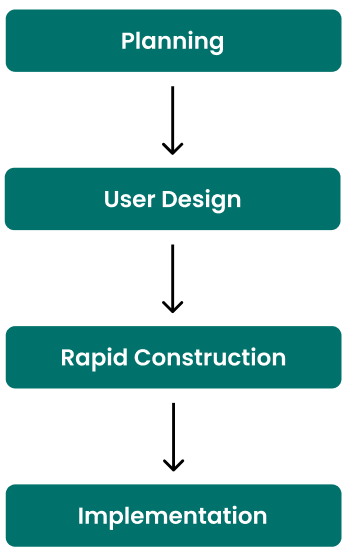
\includegraphics[width=0.3\textwidth]{images/method}
  \caption{Research Methodology Flow Diagram}
  \label{method}
\end{figure}

\noindent
\begin{enumerate}
  \item Planning
  \item[] In this stage, problem identification is carried out by discussing with stakeholders to determine the needs that are the basis for designing the system. These needs are the basis for designing and developing features in the application. From this process, a requirement specification is produced which includes the main features that must be present in the application. In addition, the target users for the system being developed are obtained, who are students of basic statistics courses.

        In addition, at this stage, the tools to be used were also agreed upon. To develop a multiplatform application, several frameworks were used, starting from Next.js for the website version, a combination of Expo and React Native for the mobile version, and Express.js as the application backend. Next.js was chosen because it has static site generation and optimized builds result in faster page loads \cite{b20}. Because of the need for fast development with the same results on Android and iOS platforms, Expo React Native is the best answer by providing a native look and fast reload \cite{b21}. Then, to store all data so that it is well organized, Express.js was chosen to build the application backend because it allows fast and efficient development \cite{b22}.

  \item User Design
  \item [] At the user design stage, an application prototype design is carried out based on the previous stage. The application design in the form of a user interface (UI) and prototype is created using the Figma tool. The prototype of this application will then be tested to evaluate its suitability to user desires. Then, all prototypes that have been tested will be adjusted again based on suggestions given by the user. The final result of this stage is an application design that includes all pages, navigation, and logical flows that will be implemented for the next stage.

        The design of the RWikiStat application can be seen in Figure~\ref{fig:design} and Figure~\ref{fig:webdesign}.
        \begin{figure}[H]
          \centering
          \begin{subfigure}{0.49\linewidth}
            \centering
            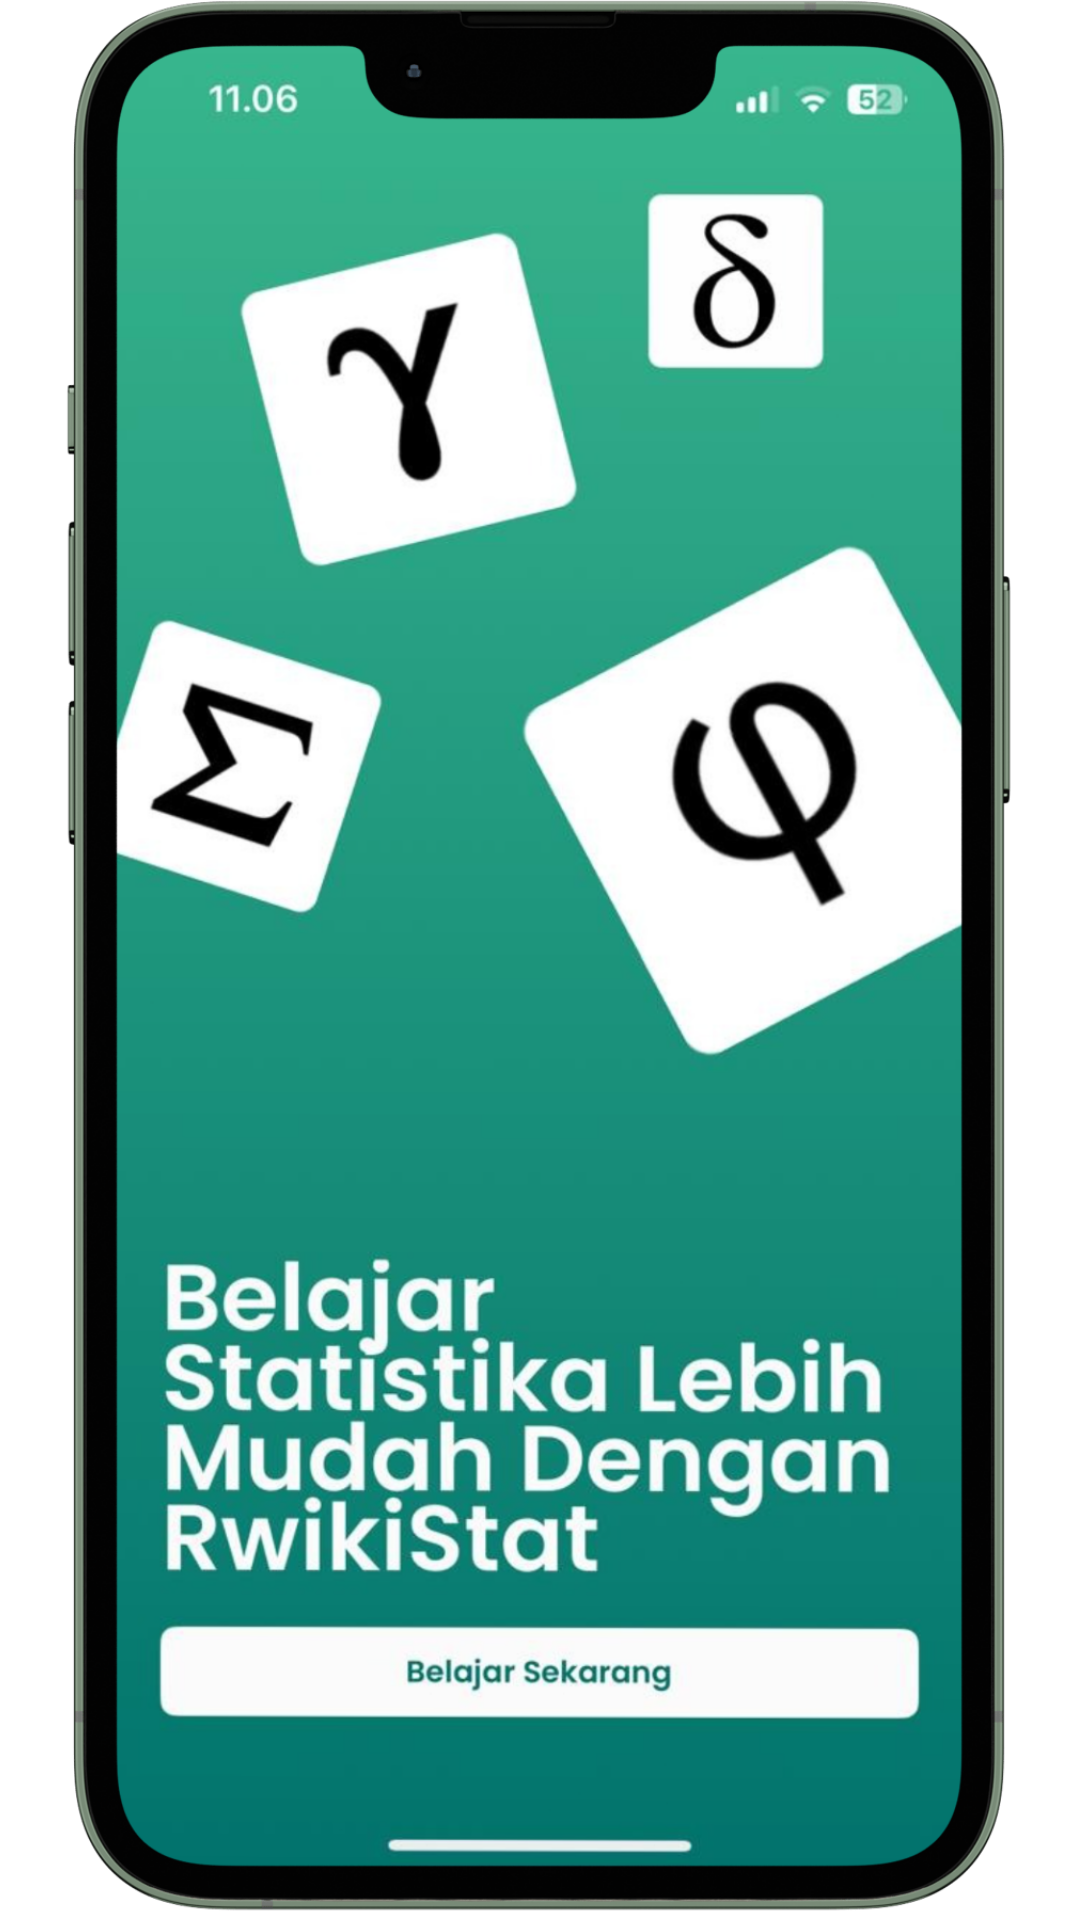
\includegraphics[width=\linewidth]{images/welcome.png}
          \end{subfigure}
          \hfill
          \begin{subfigure}{0.49\linewidth}
            \centering
            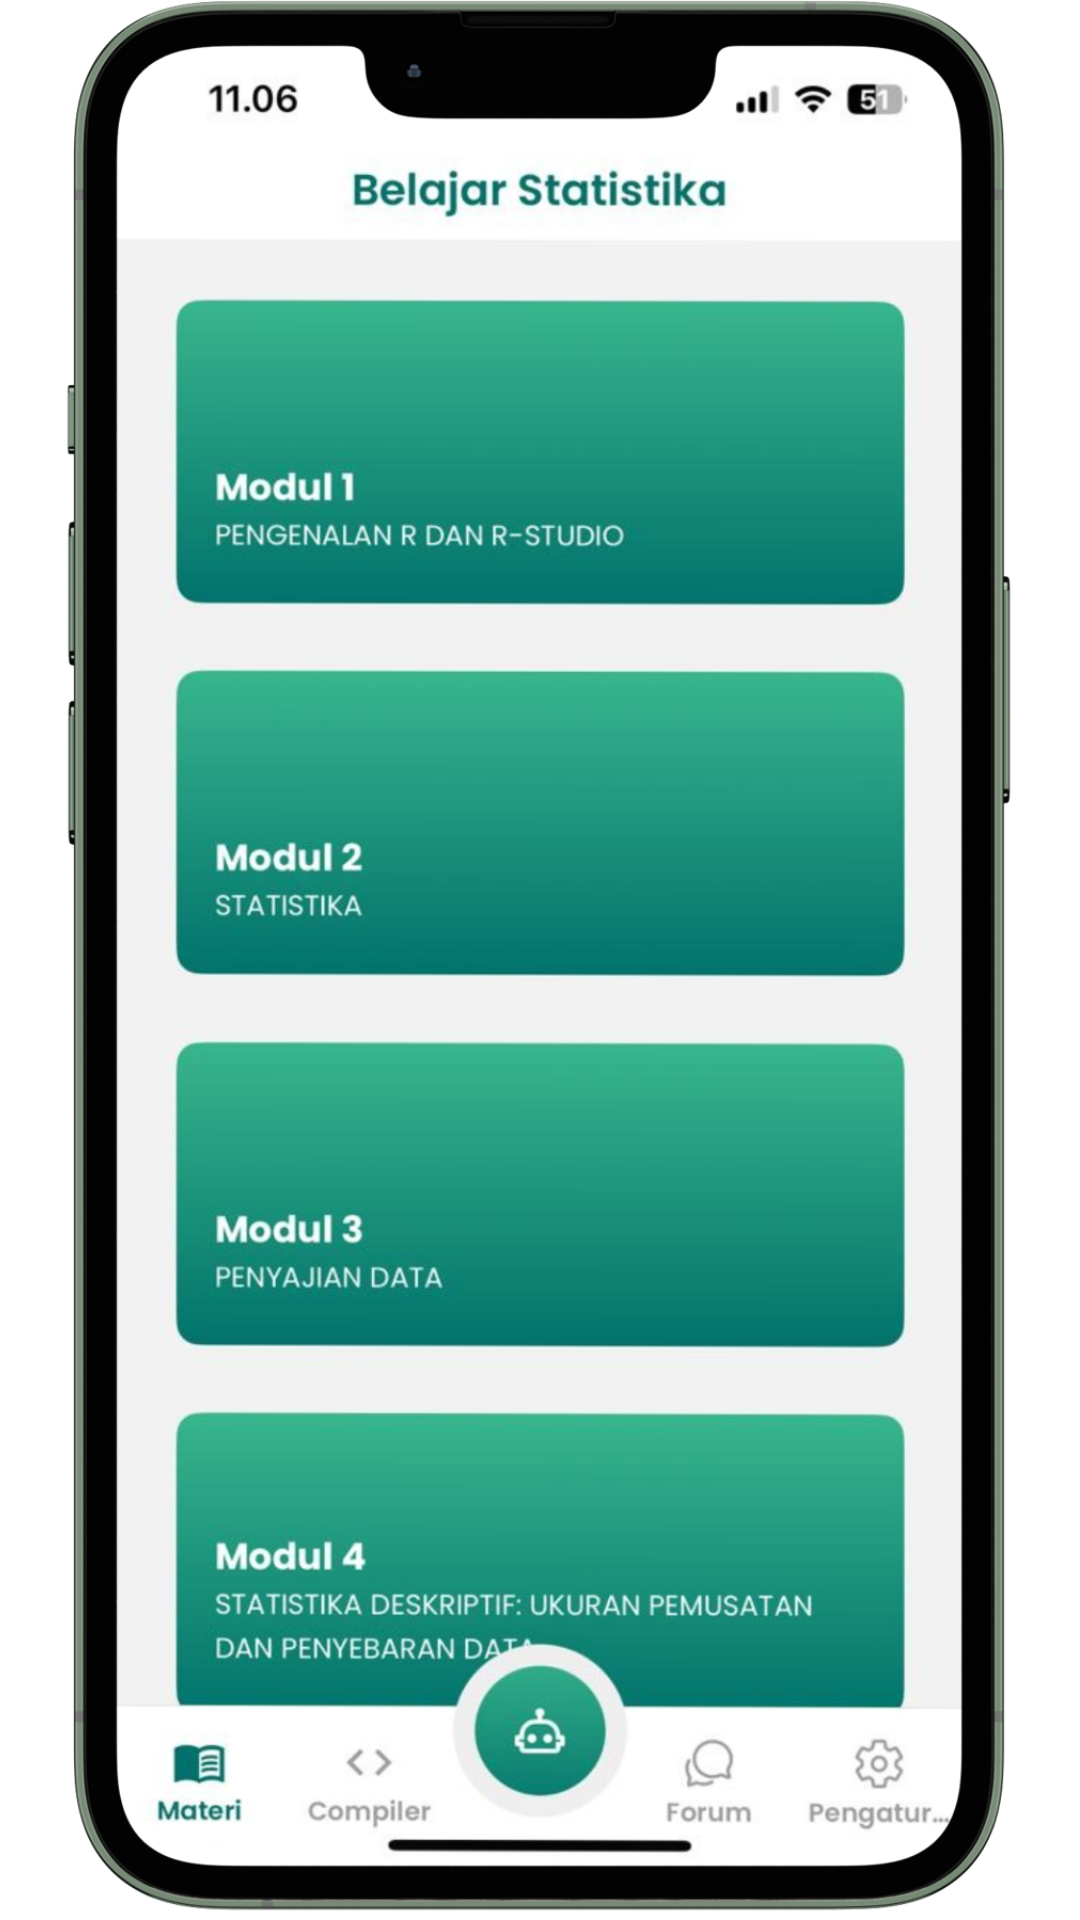
\includegraphics[width=\linewidth]{images/modul.png}
          \end{subfigure}
          \caption{RWikiStat Application Design}
          \label{fig:design}
        \end{figure}


        \begin{figure}[htb]
          \centering
          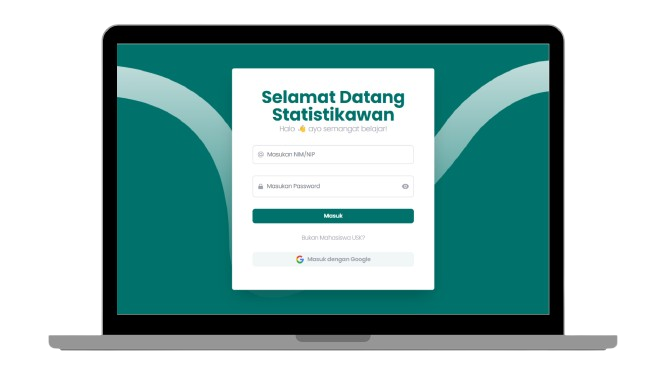
\includegraphics [width=9 cm, height=6 cm]{images/web-login.png}
          \caption{RWikiStat Web Design}
          \label{fig:webdesign}
        \end{figure}

  \item Rapid Construction
  \item [] In the rapid construction stage, the previously designed system is built. The system is built using agreed languages and frameworks, starting from database development, frontend, and backend. Through this stage, the finalized design is transformed into a usable application. In this stage, feedback collection from users is also continuously carried out to ensure that the system built is in accordance with desires.

  \item Implementation
  \item [] At the implementation stage, a thorough test is carried out on the system to ensure that there are no errors when implementing the system that has been built. Researchers use two testing methods, namely testing the system's functionality using black box testing to reduce the possibility of system defects and testing the system's usability using the Usability Metric for User Experience (UMUX) to measure the level of user satisfaction in using the system that has been built.

        The usability testing involved 22 undergraduate students who were currently enrolled in a Basic Statistics course. These participants were selected intentionally because the application was specifically designed as a learning tool for introductory statistics, making them the most relevant user group for usability evaluation.

        Prior to the usability testing, all participants were informed about the purpose of the study and voluntarily agreed to participate by providing informed consent. Personally identifiable information such as name, email, student ID, and major was collected solely for internal academic documentation in the undergraduate thesis and was not disclosed or published in this article. All usability responses were anonymized and aggregated for analysis purposes.

\end{enumerate}

\section{Results and Discussion}
\label{sect:results_discussion}

The statistics learning application, RWikiStat has been developed on all platforms starting from the website, Android and iOS with features that can help learning. RWikiStat provides a statistics learning module equipped with sample questions and code samples so that users can directly practice the statistical concepts that have been learned. In addition to trying the code samples available in each module, users can also access the compiler and try various statistical codes in the R language to strengthen their understanding. The compiler that has been equipped with Shiny integration allows users to try to visualize the desired statistical data. Furthermore, RWikiStat provides a discussion forum that can be used to ask or answer questions that are understood. Then there is also a chatbot feature so that users can ask about statistical problems without having to move to another platform.

To ensure that the system runs according to user desires, two testing processes are carried out, namely functionality testing and usability testing.

\begin{enumerate}[label=\alph*.]
  \item Functionality Testing
  \item [] Functional testing is done using black box testing to test the application in various desired scenarios. This testing is done to see the functions in the system without requiring knowledge of how the system works internally \cite{b23}. This method provides several advantages, such as rapid test case development, efficient for large code segments, and reusable testing \cite{b24}. In this study, there were 27 test scenarios performed, with all scenarios running as expected. Some of the tests performed can be seen in Table I

        \begin{table}[H]
          \centering
          \scriptsize
          \caption{Functional Testing Scenarios}
          \label{tab:functional-part1}
          \begin{tabular}{|c|p{1cm}|p{2cm}|p{2cm}|p{1cm}|}
            \hline
            \textbf{No.} & \textbf{Testing Name}   & \textbf{Scenario}                                          & \textbf{Display}                  & \textbf{Result} \\ \hline
            1            & Sign-in with student ID & Enter student ID and password, then press login button     & Redirected to main page           & Success         \\ \hline
            2            & Sign-in with Google     & Press ‘Sign in with Google’ and select account for login   & Redirected to main page           & Success         \\ \hline
            3            & Sign-in with Apple ID   & Press ‘Sign in with Apple ID’ and select account for login & Redirected to main page           & Success         \\ \hline
            4            & Access material tab     & Click the “Material” icon                                  & Redirected to material page       & Success         \\ \hline
            5            & Access compiler tab     & Click the “Compiler” icon                                  & Redirected to compiler page       & Success         \\ \hline
           
          \end{tabular}
        \end{table}

        \begin{table}[H]
          \centering
          \scriptsize
          \label{tab:functional-part2}
          \begin{tabular}{|c|p{1cm}|p{2cm}|p{2cm}|p{1cm}|}
            \hline
            \textbf{No.} & \textbf{Testing Name} & \textbf{Scenario}                                         & \textbf{Display}             & \textbf{Result} \\ \hline
             6            & Access chatbot tab      & Click the “Chatbot” icon                                   & Redirected to chatbot page        & Success         \\ \hline
             7            & Access forum tab        & Click the “Forum” icon                                     & Redirected to forum page          & Success         \\ \hline
            8            & Access settings tab     & Click the “Settings” icon                                  & Redirected to settings page       & Success         \\ \hline
            9            & Select learning module  & Select one of the module cards                             & Redirected to module + R compiler & Success         \\ \hline
            10           & Execute R/Shiny code  & Enter simple R/Shiny code to execute                      & Compilation result displayed & Success         \\ \hline
            11           & Add question to forum & Fill topic, description, photo, then press ‘Add Question’ & New question is added        & Success         \\ \hline
            12           & Logout                & Click logout icon on settings page                        & Redirected to sign-in page   & Success         \\ \hline
          \end{tabular}
        \end{table}


  \item Usability Testing
  \item [] Usability testing is done using the UMUX method to test whether the system can be understood and used by users. This method has several advantages, one of which is that this method is quite concise because it only consists of 4 questions, but still shows a high level of reliability and good validity \cite{b25}. Before conducting the test, an application test plan is first prepared which can be seen in Table~\ref{tab:test_plan}.

        \begin{table}[htbp]
          \caption{Test Plan Application}
          \label{tab:test_plan}
          \resizebox{\columnwidth}{!}{%
            \begin{tabular}{|l|}
              \hline
              \multicolumn{1}{|c|}{{\color[HTML]{333333} \textbf{Test Plan Application}}} \\ \hline
              {\color[HTML]{333333}
                \begin{tabular}[c]{@{}l@{}}
                  Scenario:                                                      \\
                  - The user opens the application.                              \\
                  - The user understands the appearance of the home page.        \\
                  - The user logs into the application.                          \\
                  - The user accesses the learning modules.                      \\
                  - The user reads the available learning modules.               \\
                  - The user downloads the available learning modules.           \\
                  - The user tries to compile R code.                            \\
                  - The user tries to ask the chatbot a question.                \\
                  - The user tries to post a question in the discussion forum.   \\
                  - The user tries to answer a question in the discussion forum. \\
                  - The user tries to save a post.                               \\
                  - The user tries to like a post.                               \\
                  - The user tries to view their post history.                   \\
                  - The user tries to delete their own question.                 \\
                  - The user tries to sign out of the application.
                \end{tabular}
              }                                                                           \\ \hline
              {\color[HTML]{333333}
                \begin{tabular}[c]{@{}l@{}}Tool:\\ - iOS Smartphone\end{tabular}
              }                                                                           \\ \hline
            \end{tabular}%
          }
        \end{table}

        Respondents will run the application according to the test plan that has been made. Respondents for this test consisted of 22 students of basic statistics courses. After that, respondents were asked to fill out a questionnaire form with questions as shown in Table~\ref{tab:umux_question_list}.

        \begin{table}[H]
          \caption{UMUX QUESTION LIST \cite{b26}}
          \label{tab:umux_question_list}
          \centering
          \renewcommand{\arraystretch}{2.2} % tinggi baris
          \begin{tabular}{|c|p{6cm}|c|} % atur lebar kolom pertanyaan
            \hline
            \textbf{No.} & \textbf{Question}                                      & \textbf{Score} \\ \hline
            1            & This application suits my needs.                       & 1 - 7          \\ \hline
            2            & I had a bad experience using this application.         & 1 - 7          \\ \hline
            3            & This application is easy to use.                       & 1 - 7          \\ \hline
            4            & I have to spend a lot of time to use this application. & 1 - 7          \\ \hline
          \end{tabular}
        \end{table}

  \item Discussion and Limitations
  \item [] The usability score obtained from the UMUX method was 88.26\%, which falls into the “Best Imaginable” category, indicating an excellent level of user satisfaction. This score suggests that RWikiStat provides a highly usable interface and effective user experience. While this score is slightly lower than EstApp, which reported 94.1\% positive responses regarding ease of use \cite{b14}, it is important to note that EstApp's evaluation was conducted using a simpler usability questionnaire through Google Forms and Likert scales, rather than a standardized tool like UMUX. Furthermore, compared to Blackburn's eLearning platform, which only reported 63\% of students perceiving quizzes as helpful without formal usability testing \cite{b15}, RWikiStat clearly demonstrates a more rigorous and reliable evaluation approach. These comparisons suggest that RWikiStat not only delivers high user satisfaction, but also surpasses many educational platforms in terms of methodological robustness in usability assessment.
  
  In addition to the quantitative score, qualitative feedback was also collected from the 22 student respondents. All participants reported a positive experience while using the application. They appreciated the ease of navigating through the modules, the usefulness of the integrated R compiler, and the presence of the chatbot which allowed them to ask questions directly within the app. Several respondents highlighted that the application helped them better understand statistical concepts through hands-on code practice and instant feedback.

	Despite the positive results, this study has several limitations. First, the number of respondents was limited to 22 students, which may not represent the broader user base. Second, all respondents were students enrolled in the same course and institution, which may introduce contextual bias. Third, the usability test only measured short-term interactions with the application, without assessing long-term engagement or retention of statistical concepts.

  Future work may consider expanding the demographic scope of participants, conducting longitudinal usability evaluations, and comparing user engagement and learning outcomes across different educational tools in the same domain.

\end{enumerate}

After testing using the UMUX method, the test result data is processed following these steps:
\begin{itemize}
  \item Each odd-numbered item is calculated using the formula [user score- 1], while even-numbered items are calculated using the formula [7- user score].
  \item The scores of each item filled in by the user are added up first, then divided by 24 (the maximum score value).
  \item The result of the division is multiplied by 100.
  \item Furthermore, the value is averaged for all users.
  \item The UMUX score obtained is assessed on a scale of 0-100, according to general assessment standards\cite{b27}.
\end{itemize}
 
The outcomes of the usability evaluation, which was carried out using the UMUX method to assess user satisfaction and system usability can be seen in Table~\ref{tab:umux_results}.

\newpage
\begin{table}[htbp]
  \caption{UMUX Testing and Evaluation Results for the RWikiStat Application}
  \label{tab:umux_results}
  \resizebox{\columnwidth}{!}{%
    \begin{tabular}{|l|c|c|c|c|c|}
      \hline
      \multirow{2}{*}{\textbf{Respondent}}   & \multicolumn{4}{c|}{\textbf{Question Number}} & \multirow{2}{*}{\textbf{Final Score}}                                   \\ \cline{2-5}
                                             & \textbf{1}                                    & \textbf{2}                            & \textbf{3} & \textbf{4} & ~     \\ \hline
      Student 1                              & 7                                             & 1                                     & 7          & 1          & 100   \\ \hline
      Student 2                              & 4                                             & 1                                     & 7          & 1          & 87,5  \\ \hline
      Student 3                              & 4                                             & 1                                     & 6          & 2          & 79,17 \\ \hline
      Student 4                              & 7                                             & 1                                     & 7          & 3          & 91,67 \\ \hline
      Student 5                              & 6                                             & 2                                     & 5          & 3          & 75    \\ \hline
      Student 6                              & 7                                             & 1                                     & 7          & 1          & 100   \\ \hline
      Student 7                              & 7                                             & 2                                     & 7          & 1          & 95,83 \\ \hline
      Student 8                              & 7                                             & 1                                     & 7          & 1          & 100   \\ \hline
      Student 9                              & 7                                             & 1                                     & 7          & 1          & 100   \\ \hline
      Student 10                             & 7                                             & 2                                     & 6          & 2          & 87,5  \\ \hline
      Student 11                             & 7                                             & 1                                     & 7          & 2          & 95,83 \\ \hline
      Student 12                             & 7                                             & 2                                     & 5          & 2          & 83,33 \\ \hline
      Student 13                             & 7                                             & 1                                     & 7          & 1          & 100   \\ \hline
      Student 14                             & 5                                             & 1                                     & 7          & 5          & 75    \\ \hline
      Student 15                             & 7                                             & 1                                     & 7          & 4          & 87,5  \\ \hline
      Student 16                             & 7                                             & 1                                     & 7          & 1          & 100   \\ \hline
      Student 17                             & 6                                             & 1                                     & 7          & 1          & 95,83 \\ \hline
      Student 18                             & 5                                             & 1                                     & 7          & 1          & 91,67 \\ \hline
      Student 19                             & 4                                             & 1                                     & 4          & 2          & 70,83 \\ \hline
      Student 20                             & 6                                             & 2                                     & 6          & 6          & 66,67 \\ \hline
      Student 21                             & 7                                             & 1                                     & 7          & 5          & 83,33 \\ \hline
      Student 22                             & 6                                             & 1                                     & 6          & 4          & 75    \\ \hline
      \multicolumn{5}{|c|}{\textbf{Average}} & \textbf{88.26}                                                                                                          \\ \hline
    \end{tabular}%
  }
\end{table}

Based on the test results in Table~\ref{tab:umux_results}, an average value of 88.26\% was obtained. This shows that the RWikiStat application has an interpretation score of "Best Imaginable" with a grade of "A" using the UMUX calculation method.



\section{Conclusions and Suggestions}
\label{sect:conclusion}

In this paper, we introduced RWikiStat, an interactive learning application designed to enhance student engagement in introductory statistics courses. Through its integrated learning tools and interactive features, RWikiStat effectively supports both conceptual understanding and hands-on practice.
Functionality testing using the black-box method confirmed that all features performed as intended. Meanwhile, usability evaluation through the UMUX method yielded a satisfaction score of 88.26\%, which falls under the category of “Best Imaginable” (grade A), indicating strong acceptance from students who participated in the testing. 

While these results are encouraging, it is important to recognize that usability alone does not fully reflect the educational impact of a learning application. Future studies should assess the application’s effect on measurable learning outcomes, such as improved performance in assessments or increased conceptual mastery, to gain a deeper understanding of its effectiveness in supporting student learning. 

Pedagogically, RWikiStat reflects principles of constructivist learning, as it encourages students to explore, experiment, and build knowledge through interactive features. The inclusion of a discussion forum and independent learning modules also aligns with blended learning models, supporting flexibility and peer-to-peer engagement beyond the confines of traditional classrooms. 

Moving forward, several enhancements are planned to expand the educational and technical reach of the application. These include the addition of multi-language support to accommodate diverse learners, offline access to improve usability in areas with limited internet connectivity, and integration with learning management systems (LMS) to enable personalized feedback and continuous monitoring of student progress. These future developments are intended to strengthen both the pedagogical value and the accessibility of RWikiStat, paving the way for broader adoption in statistics education.



\balance

\begin{thebibliography}{00}

  \bibitem{b1} Ririen, Deci, and Dewi Hartika. "Identifikasi Kesulitan Belajar Mahasiswa pada Mata Kuliah Statistika Selama Masa Pandemi Covid-19." \textit{Jurnal Ilmiah Universitas Batanghari Jambi} 21.1 (2021): 148-155. \href{http://dx.doi.org/10.33087/jiubj.v21i1.1236}{http://dx.doi.org/10.33087/jiubj.v21i1.1236}

  \bibitem{b2} Wild, Chris J., and Maxine Pfannkuch. "Statistical thinking in empirical enquiry." \textit{International Statistical Review} 67.3 (1999): 223-248. \href{https://doi.org/10.1111/j.1751-5823.1999.tb00442.x}{https://doi.org/10.1111/j.1751-5823.1999.tb00442.x}

  \bibitem{b3} Uchima-Marin, Cristian, et al. "Integration of Technological Tools in Teaching Statistics: Innovations in Educational Technology for Sustainable Education." \textit{Sustainability} 16.19 (2024): 8344. \href{https://doi.org/10.3390/su16198344}{https://doi.org/10.3390/su16198344}

  \bibitem{b4} Wilson, Stephanie Gray. "The flipped class: A method to address the challenges of an undergraduate statistics course." \textit{Teaching of Psychology} 40.3 (2013): 193-199. \href{https://doi.org/10.1177/0098628313487461}{https://doi.org/10.1177/0098628313487461}

  \bibitem{b5} Talan, Tarik. "The effect of mobile learning on learning performance: A meta-analysis study." \textit{Kuram Ve Uygulamada Egitim Bilimleri} 20.1 (2020): 79-103.

  \bibitem{b6} Subianto, Muhammad, and Hizir Sofyan. "Interactive statistics learning with RWikiStat." \textit{2010 International Conference on Networking and Information Technology}. IEEE, 2010. \href{http://dx.doi.org/10.12738/jestp.2020.1.006}{http://dx.doi.org/10.12738/jestp.2020.1.006}

  \bibitem{b7} Sofyan, Hizir, Edi Muttaqin, and Muhammad Subianto. "RWikiStat 2.0: A Web Based Statistical Learning System (Session 1B (IASC-ARS))." \textit{Proceedings of the Symposium of Japanese Society of Computational Statistics} 26. Japanese Society of Computational Statistics, 2012. \href{https://doi.org/10.1109/ICNIT.2010.5508452}{https://doi.org/10.1109/ICNIT.2010.5508452}

  \bibitem{b8} Sofyan, Hizir, et al. "Analisis Kepuasan Pengguna Aplikasi RWikiStat 3.0." \textit{Journal of Data Analysis} 2.2 (2020): 80-87. \href{https://doi.org/10.20551/jscssymo.26.0\_149}{https://doi.org/10.20551/jscssymo.26.0\_149}

  \bibitem{b9} Sarkar, Subrata, Sanjay Mohapatra, and Jayaraman Sundarakrishnan. "Assessing impact of technology based digital equalizer programme on improving student learning outcomes." \textit{Education and Information Technologies} 22.1 (2017): 195-213. \href{https://doi.org/10.1007/s10639-015-9434-0}{https://doi.org/10.1007/s10639-015-9434-0}

  \bibitem{b10} Arain, Aijaz Ahmed, et al. "An analysis of the influence of a mobile learning application on the learning outcomes of higher education students." \textit{Universal Access in the Information Society} 17 (2018): 325-334. \href{https://doi.org/10.1007/s10209-017-0551-y}{https://doi.org/10.1007/s10209-017-0551-y}

  \bibitem{b11} López-Pérez, María V., et al. "The influence of the use of technology on student outcomes in a blended learning context." \textit{Educational Technology Research and Development} 61 (2013): 625-638. \href{https://doi.org/10.1007/s11423-013-9303-8}{https://doi.org/10.1007/s11423-013-9303-8}

  \bibitem{b12} Ansong-Gyimah, Kwame. "Students’ Perceptions and Continuous Intention to Use E-Learning Systems: The Case of Google Classroom." \textit{International Journal of Emerging Technologies in Learning (iJET)} 15.11 (2020): 236-244. \href{https://doi.org/10.3991/ijet.v15i11.12683}{https://doi.org/10.3991/ijet.v15i11.12683}

  \bibitem{b13} Zhang, Qi, and Zhonggen Yu. "A literature review on the influence of Kahoot! on learning outcomes, interaction, and collaboration." \textit{Education and Information Technologies} 26.4 (2021): 4507-4535. \href{https://doi.org/10.1007/s10639-021-10459-6}{https://doi.org/10.1007/s10639-021-10459-6}

  \bibitem{b14} Quiñones, Daniela, et al. "Innovating Statistics Education: The Design of a Novel App Using Design Thinking." \textit{Applied Sciences} 14.18 (2024): 8515. \href{https://doi.org/10.3390/app14188515}{https://doi.org/10.3390/app14188515}

  \bibitem{b15} Blackburn, Greg. "Effectiveness of eLearning in statistics: Pictures and stories." \textit{E-Learning and Digital Media} 12.5-6 (2015): 459-480. \href{https://doi.org/10.1177/2042753016653704}{https://doi.org/10.1177/2042753016653704}

  \bibitem{b16} González, José A., et al. "Assessing Shiny apps through student feedback: Recommendations from a qualitative study." \textit{Computer Applications in Engineering Education} 26.5 (2018): 1813-1824. \href{https://doi.org/10.1002/cae.21932}{https://doi.org/10.1002/cae.21932}

  \bibitem{b17} Thai, Hong-Danh, Yeong-Seok Seo, and Jun-Ho Huh. "Enhanced Efficiency in SMEs Attendance Monitoring: Low Cost Artificial Intelligence Facial Recognition Mobile Application." \textit{IEEE Access} (2024). \href{http://dx.doi.org/10.1109/ACCESS.2024.3504858}{http://dx.doi.org/10.1109/ACCESS.2024.3504858}

  \bibitem{b18} Balbontin, Pinky A., et al. "Electronic document archiving system." Diss. 2009.

  \bibitem{b19} Alguidano Jr, Ramon A., et al. "Scientia et Fides."

  \bibitem{b20} Svedas, Egidijus. "Building an application using Next.js." (2024).

  \bibitem{b21} Nitschke, Marlies, et al. "Refinement and usability analysis of an eHealth app for ankylosing spondylitis as a complementary treatment to physical therapy: Development and usability study." \textit{JMIR Formative Research} 7 (2023): e47426. \href{https://doi.org/10.2196/47426}{https://doi.org/10.2196/47426}

  \bibitem{b22} Azkarin, Varinia, Rangga Gelar Guntara, and Oding Herdiana. "Development of a REST API for Human Resource Information System for Employee Referral Management Domain Using the Express JS Framework and Node.js." \textit{Journal of Scientific Research, Education, and Technology (JSRET)} 2.3 (2023): 1085-1094. \href {https://doi.org/10.58526/jsret.v2i3.199}{https://doi.org/10.58526/jsret.v2i3.199}

  \bibitem{b23} Kumar, Manish, Santosh Kumar Singh, and R. K. Dwivedi. "A comparative study of black box testing and white box testing techniques." \textit{International Journal of Advance Research in Computer Science and Management Studies} 3.10 (2015).

  \bibitem{b24} Khan, Mohd Ehmer, and Farmeena Khan. "A comparative study of white box, black box and grey box testing techniques." \textit{International Journal of Advanced Computer Science and Applications} 3.6 (2012). \href{http://dx.doi.org/10.14569/IJACSA.2012.030603}{http://dx.doi.org/10.14569/IJACSA.2012.030603}

  \bibitem{b25} Lewis, James R. "Measuring perceived usability: The CSUQ, SUS, and UMUX." \textit{International Journal of Human–Computer Interaction} 34.12 (2018): 1148-1156. \href{https://doi.org/10.1080/10447318.2017.1418805}{https://doi.org/10.1080/10447318.2017.1418805}

  \bibitem{b26} Lewis, James R., and Jeff Sauro. "Usability and user experience: Design and evaluation." \textit{Handbook of Human Factors and Ergonomics} (2021): 972-1015. \href{https://doi.org/10.1002/9781119636113.ch38}{https://doi.org/10.1002/9781119636113.ch38}

  \bibitem{b27} Finstad, Kraig. "The usability metric for user experience." \textit{Interacting with Computers} 22.5 (2010): 323-327. \href{https://doi.org/10.1016/j.intcom.2010.04.004}{https://doi.org/10.1016/j.intcom.2010.04.004}

\end{thebibliography}

\end{document}